\chapter{Le statut de dhimmi de la
naissance de l’islam aux Omeyyades}

\mn{Séance 2 (MarieCarmen Smyrnelis) du 24 janvier}


\section{Bibliographie}

\begin{itemize}
    \item CAHEN Claude,
Islam, des origines au début de l’Empire ottoman , Paris, Hachette, coll. « Pluriel », 2011.
    \item 
GAUDEUL
Jean Marie, Disputes ? Ou rencontres ?, l’islam et le christianisme au fil des siècles, Rome,
PISAI, coll. « Studi arabo islamici », n 12, 1998, 2 volumes.
    \item 
HOURANI Albert,
Histoire des peuples arabes , Paris, Seuil, coll. « Points », 1993.
    \item 
LEWIS Bernard,
Les Arabes dans l’histoire , Paris, Flammarion, « Champs », 1993.
    \item 
RODINSON Maxime,
Les Arabes, Paris, PUF, coll. « Quadrige », 2002.
\end{itemize}


\section{Les débuts de l’islam}

\subsection{la péninsule arabique à la veille de l'apparition de l'islam}

\paragraph{une lutte entre l'empire bysantin et l'empire sassanide}
\begin{Def}[Empire]
Ce qui caractérise l'empire, c'est l'hétérogéneité des peuples qui la compose. 
\end{Def}

 \subsection{Repères chronologiques}
 \begin{itemize}
   \item	570-580 : naissance de Mahomet à La Mecque
\item 	622 : installation à Médine (Hégire)
\item 628 : pèlerinage annuel à la Mecque négocié avec les autorités.
\item 	630 : conquête de La Mecque
\item 	632 : mort de Mahomet
 \end{itemize}

\begin{figure}[h!]
    \centering
        \sidecaption{lorian Louis, Atlas historique du Moyen-Orient, Paris, Autrement, 2020, p. 33}
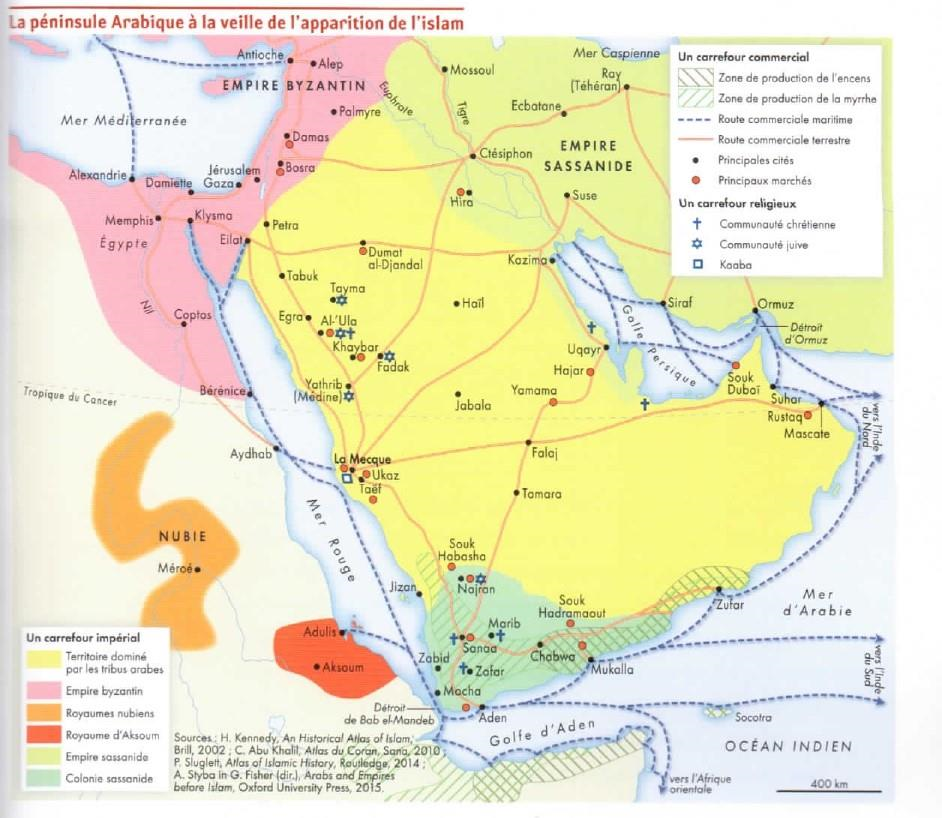
\includegraphics[width=\textwidth]{HistoireIslamMediterranee/Images/PeninsuleArabe.png}

    \label{fig:my_label}
\end{figure}


\paragraph{ce qu'en disent les historiens} A Médine, il part probablement à la demande des Médinois, s'impose pour son jugement. Fonde l'\textit{umma}. 

\paragraph{Juxtaposition de l'Umma avec les tribus} chaque tribu garde ces droits mais face à Mohammed, on suit la loi.

\paragraph{Première "constitution" médinoise} relation des membres entre eux, comment on traite en dehors de l'\textit{umma}. 
La foi va remplacer le lien de sang, nouveau lien. La source de l'autorité passe de la vue publique à Dieu.

\paragraph{L'umma prend une dimension de l'umma} Mohammed fonde à la fois une foi mais aussi un corps politique. 
\begin{Def}[théocratie]
    mélange politique et religieux
\end{Def}
Mais on plaque la politique actuelle alors que c'est une réalité bien différente.

\paragraph{de l'attaque des caravanes à l'extension du territoire} 

\paragraph{630 - Mecque : des affaires politiques avec les tribus} mais pas religieux qui reste quelque chose d'individuel dans un premier temps.  \textsc{Une vraie question pour la suite du collectif et de l'individuel et en particulier pour la conversion. }
Au début, la tribu accepte de ne pas attaquer les musulmans, elle accepte de payer l'impôt religieux mais elle n'est pas obligée de se convertir.

L'accord se place toujours avec Mahomet jusqu'à sa mort.

\paragraph{632 mort de Mahomet} les difficultés commencent.  Il n'avait pas laissé d'instructions de succession. 


\section{Les Rasidun les « bien guidés », successeurs de Mahomet et califes}

 

\paragraph{de nombreuses questions à la mort du Prophète} Qui va avoir l'autorité ? Comment gérer le statut des non musulmans ? pratique du Coran

\paragraph{Alors que ce monde connaît un bouleversement politique} Avec un embryon étatique. Certains historiens considèrent l'empire arabe à la mort de Mahomet.


\paragraph{les Rasidun (632-661) : successeurs de Mahomet}
\begin{itemize}
  \item 	Abu Bakr (632-634)\sn{beau-Père de Mahommed, déput de l'institution du califat}
\item 	Umar (634-644)
\item 	Uthman (644-656)
\item 	Ali (656-661)
\item 	les Omeyyades (661-749) => transfert de la capitale à Damas
\end{itemize}

\paragraph{Abu Bakr} Chef d'une communauté et chef d'un territoire. Pas trop de difficultés du fait de la durée de deux ans

\paragraph{Umar} Cela se complique. Est tué par un esclave persan. comprend la question Islam et Arabie, alors que l'Islam rentre en Perse.  

\paragraph{Des révoltes} de tribus s'opposant au choix d'Abu Bakr et Uman. Pour calmer ces tribus, l'extension du territoire est nécessaire.

\paragraph{Question de l'Empire} avec la taille du territoire, se passe la question de l'acceptation culturelle et religieuse locale.
\begin{itemize}
    \item \item 	633-637 : conquête de la Syrie
\item 	639-642 : conquête de l’Egypte. Se passe bien du fait que les coptes en ont assez de Byzance. Du côté de Byzance, on a une armée de mercernaires peu motivés d'appliquer une loi peu acceptée par les populations locales. 
\item 	634-652 : conquête de la Perse. 

\end{itemize}

\paragraph{utilisation du désert} pour se retirer et communiquer. Installation des villes à la frontière du désert, villes d'appui, où les arabes sont majoritaires. Dans ces villes, \textit{amsar}, l'arabe est la langue. Dans le reste, les musulmans sont minoritaires.   
C'est assez classique dans un empire, où la culture de l'empire est minoritaire.

\begin{Ex}[Fustat]
Ils quittent Alexandrie et fondent Fustat.  Ces villes nouvelles, \textit{amsar}, sont encouragées par des taxes. C'est une expansion \textit{arabe} et pas forcément de l'Islam, puisque les tribus arabes ne sont pas toutes islamisées.
\end{Ex}

\begin{Ex}[Bosra en Syrie]
\begin{marginfigure}
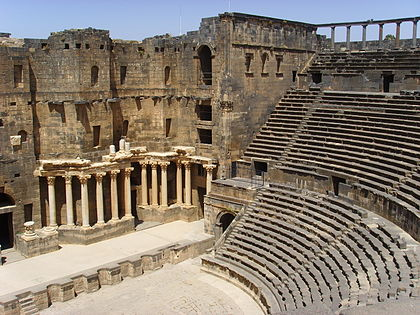
\includegraphics[width=\textwidth]{HistoireIslamMediterranee/Images/TheaterBosra2.jpg}
\end{marginfigure}
    Avait déjà une population arabe importante avant la conquête. 
\end{Ex}

\paragraph{Respect des cultures locales} D'abord, on préserve les cultures locales. L'idée d'une conversion totale ne se pose pas, en dehors de l'Arabie. On demande la soumission et en échange, on a la protection. 

\paragraph{Propriété respectée} sauf si propriété d'un disparu ou propriété de l'Etat. Mais uniquement au début. 

\paragraph{Un impôt de soumission} Il est interdit quand on n'est pas arabe, de s'habiller comme un arabe. 
\begin{Def}[mawali]
    ce sont des non arabes convertis, normalement égaux, ne payent pas de textes mais considérés comme socialement inférieurs.
\end{Def}


\paragraph{Uthman} Arrêt de la conquête. Se pose le problème de l'organisation. 

\paragraph{de fortes révoltes} pas vraiment personnel contre Uthman ni religieuse mais des enjeux de pouvoir. Uthman avait moins de légitimité et apparait faible.
Les nomades se révoltent depuis l'Egypte et depuis Médine contre les hommes de la Mecque.  

\begin{Prop}
A cette époque la relation et la fidélité sont toujours individuels au calife. 
\end{Prop}

\paragraph{L'assassinat de Uthman } par un esclave perse. Sans doute pour un problème politique. Annonce pour certains historiens la lutte de la Perse.


\paragraph{Ali} proclamé Calife à Médine. Pour des raisons politiques, il démet les fonctionnaires nommés par Uthman mais il ne punit pas les meurtriers de Uthman. Il est donc accusé d'avoir une responsabilité dans sa mort.

\paragraph{Bataille de Bassora} Ali la gagne mais sort affaibli. Le gouverneur de la Syrie, pour venger Uthman, lève une armée et attaque Ali. 

\paragraph{} Le gouverneur de Syrie met le coran sur les lances. Ali est tué et son fils renonce au califat. Le gouverneur de Syrie devient Calife Omeyyade.


\paragraph{sous les rasidun}


\section{La dynastie des Omeyyades}


\paragraph{le Calife  Muʿāwiyah ibn ʾAbī Sufyān} crée la dynastie. Centraliser le pouvoir. 

\paragraph{transfert de la capitale de Médine à Damas} On s'éloigne de l'Arabie. L'influence des arabes en Syrie devient très importante. On contrôle la \Med orientale. Même si les Omeyyades restent attachés au désert (cf qsars, chateau).

\paragraph{La \textit{chura}} Muʿāwiyah crée un conseil consultatif et executif, le conseil des tribus. Il s'appuie sur des instances qu'il créé. Via les gouverneurs et la \textit{chura}, il gouverne sur la totalité du territoire.

\paragraph{Le personnel de l'empire byzantin ou perse reste} 



\begin{figure}[h!]
    \centering
      \sidecaption{\textsc{De Muhammed aux Omeyyades : expansion et division de l'Islam}. Florian Louis, Atlas historique du Moyen-Orient, Paris, Autrement, 2020, p. 37.
      Certaines batailles vont avoir un rôle important dans le positionnement de l'Islam}
   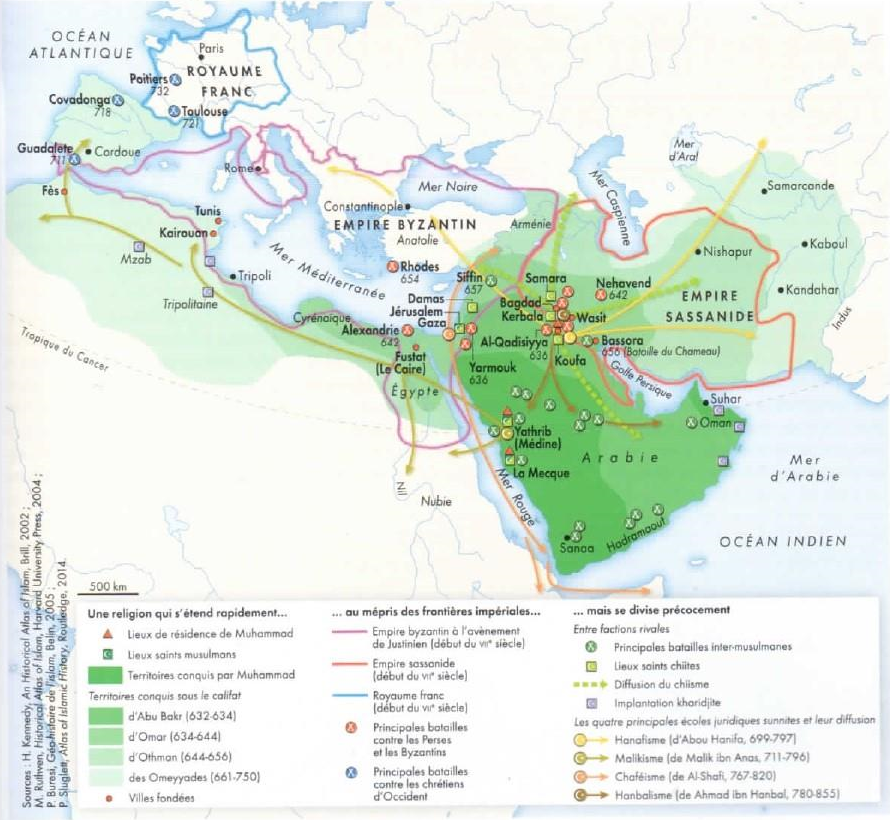
\includegraphics[width=\textwidth]{HistoireIslamMediterranee/Images/ExpansionMusulmane.png}
  
    \label{fig:my_label}
\end{figure}
\paragraph{Principales conquêtes}
\begin{itemize}
   \item 	696 : Chute de Carthage
\item 	710 : débarquement en Espagne, par le soutien des tribus berbères
\item 	732 : bataille dite de Poitiers (Omeyyades mis en échec par Charles Martel)
\end{itemize}
Ils vont essayer de prendre Bysance à deux reprises, échec.

\paragraph{Son successeur,Yazīd Ier} avec des dissensions importantes. Développement d'une civilisation brillante. Une minorité d'arabe dirigeant une majorité non musulmane.

\paragraph{des conversions pour des raisons diverses} Cela peut être pour s'intégrer dans l'élite, la simplicité de l'Islam avec des modalités simples, pour des raisons fiscales. Les zoroastriens se convertissent plus facilement que les chrétiens. 
A partir d'un certain moment, pour des raisons économiques, les Omeyyades découragent les conversions. 

\paragraph{Les partisans d'Ali} Les \textit{Mawalis} qui se sont convertis mais ne dépendant pas d'une tribu arabe (berbere, persans, Iraniens,...), surtout dans les \textit{amsar}. Ils ont une paie inférieure,... Leur poids démographique augmente. Ils vont trouver une traduction religieuse dans le Chi'isme : ils manifestent d'une façon politique contre le pouvoir établi. Ce ne sont pas uniquement des non arabes qui sont chiites. \textit{Une complexité} avec des mariages mixtes (avec esclaves). La révolte boue. 
Ce n'est donc pas qu'une révolte religieuse mais sociale et politique. Les "demi-arabes" vont se révolter et soutenir \textit{Ali} et ses descendants. 

\paragraph{Consolidation du pouvoir} Monnaie (Dihram et Dinar)... 


\section{Le statut de dhimmi}
